\chapter{CouchDB}
\label{couchdb}
This chapter covers an introduction to \emph{Apache CouchDB}\footnote{\url{http://couchdb.apache.org}}. Thereafter,  For further information, see~\cite{Anderson10}.\\
CouchDB is a so-called \emph{NoSQL} database implemented in \emph{Erlang}\footnote{\url{http://www.erlang.org}}, whose aim is primarily facilitating horizontal scaling (distributed database). In contrast to common relational databases, it does not use tables to store data, but documents expressed in the \emph{JavaScript Object Notation} (JSON). Hence, a database in CouchDB consists of a set of documents. The advantage of store data as documents is simple extensibility and processing of the database.

\section{RESTful API}
\label{couchdb:restfulapi}
Since CouchDB provides a RESTful\footnote{\url{http://en.wikipedia.org/wiki/Restful}} API, and each of CouchDB's documents has its own, unique Uniform Resource Identifier (URI), every document can be retrieved and manipulated via the HTTP methods POST, GET, PUT and DELETE. Therefore, CouchDB basically also acts as web server, wherefore establishing a communication between CouchDB and a client is pretty straight-forward and simple.\\
Furthermore, CouchDB provides a web-based built-in administration interface called \emph{Futon}, supporting the creation, manipulation, and deletion of databases, views, and documents.

\section{Replication}
One of CouchDB's most famous features is \emph{replication}. This feature synchronizes two copies of the same database, allowing low latency access to data. Remarkably, this can also be done by appropriate HTTP methods. Therefore, creating backups of the database is a pretty simple task. Moreover, as stated later in chapter~\ref{couchapp}, since CouchApps are so-called \emph{Design documents}, which are in turn also common CouchDB documents, a backup of the database also applies to its CouchApps.

\section{Change Notifications}
\label{couchdb:changesfeed}
Another CouchDB feature is its \emph{changes feed}. By the use of this feature, applications can avoid polling of the database. In this context, polling refers to the repeated checking for changes in the database. However, in client-server scenarios, this may lead to a considerable increase of the network traffic.\\
Consequently, CouchDB's changes notifies all registered clients, when certain changes of documents occur, making polling unnecessary.

\section{Documents in CouchDB}
\label{couchdb:documents}
As already mentioned, a CouchDB database consists of a set of documents expressed in JSON. A document is self-containing, i.e. its schema information is contained in itself.\\
A CouchDB document might look like the following:
\begin{lstlisting}[language=json]
{
	"_id" : "albert_einstein",
	"_rev" : "1-dadc79bfe0af3d535d285d88b6e2df07",
	"Name" : "Albert Einstein",
	"Born" : 
	{
		"Year" : 1879, 
		"City" : "Ulm"
	},
	"Nobel Prize winner" : true,
	"Fields" : ["Physics"],
	"Address" : null
}
\end{lstlisting}
The attributes \emph{\_id} and \emph{\_rev} are both mandatory. The former has to be a unique key for the document, while the latter is the revision, which gets updated by each change of the document.\\
In addition to these mandatory attributes, each document may contain further attributes of one of the following types:
\begin{description}
\item[Number] An integer or even a decimal number. See the "Year" attribute of the example document.
\item[String] An arbitrary sequence of characters, enclosed by quotation marks. See the "Name" attribute of the example document.
\item[Boolean] Either \emph{true} or \emph{false}. See the "Nobel Prize winner" attribute of the example document
\item[Array] A sequence of arbitrary JSON objects enclosed by square brackets. See the "Fields" attribute of the example document.
\item[Object] A set of key-value-pairs enclosed by curly brackets, whereas the key has to be a string and the value can be of any of the listed types. See the "Born" attribute of the example document.
\item[null] Not a type, but represents an "empty value" or "nothing". See the "Address" attribute of the example document.
\end{description}
Furthermore, in CouchDB, documents can have attachments, i.e. arbitrary files (e.g. *.html and *.js files) can be attached to documents. These attachments get their own URL by which they are accessible and manipulable.

\section{Querying CouchDB}
\label{couchdb:query}
While in relational databases, data sets are queried and manipulated by the Structured Query Language (SQL), CouchDB uses so-called \emph{map} and \emph{reduce} functions, known as MapReduce.\\
The map function is invoked for each of the source's documents. Because of the independence of these function applications, this can be done in parallel enabling horizontal scaling. Map functions can emit an arbitrary number of key-value-pairs, hence, the may, for example sort out certain documents to implement a filter operator.\\
All key-value-pairs emitted by the map functions are distributed into certain groups, which are determined by their keys, i.e. all key-value-pairs with the same key are allocated to the same group. Subsequently, the reduce function is called once for each group with each group as its argument. This can also be done independently and in parallel.\\
In CouchDB, a combination of map and reduce function is called \emph{view}. Figure~\ref{img:mapreduce} shows an exemplary definition of a view, grouping a list of scientists (documents) by their scientific field (in the map function) and counting the scientists per field (in the reduce function).
\begin{figure}[h!]
\centering
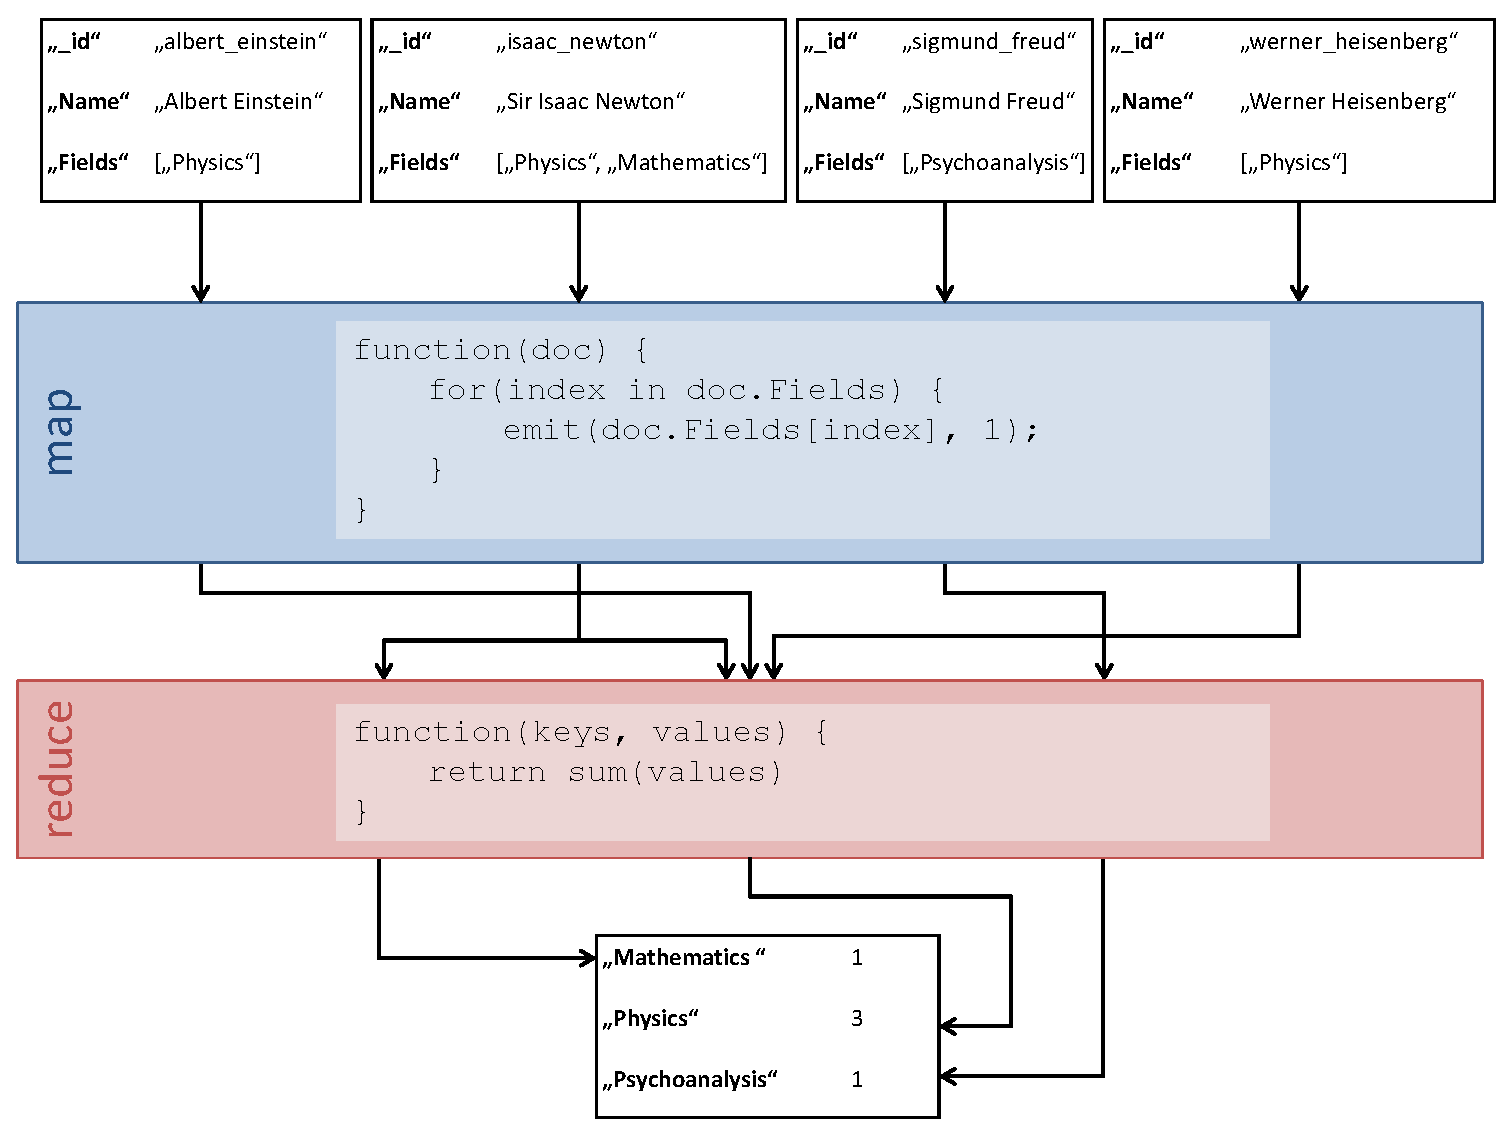
\includegraphics[width=1.0\columnwidth]{images/mapreduce.pdf}
\caption{Definition of a view by MapReduce to count the scientists per field}
\label{img:mapreduce}
\end{figure}

\section{Design documents}
\label{designdocument}
Queries can be either temporary or they can be stored to the database, whereas a query is stores as a \emph{Design document}, having an attribute "views", which contains the map as well as the reduce function (see Figure~\ref{img:couchdbviewdocument}). In Futon, stored views can be selected in the database view as shown in Figure~\ref{img:couchdbviewselection}.\\
\begin{figure}[h!]
\centering
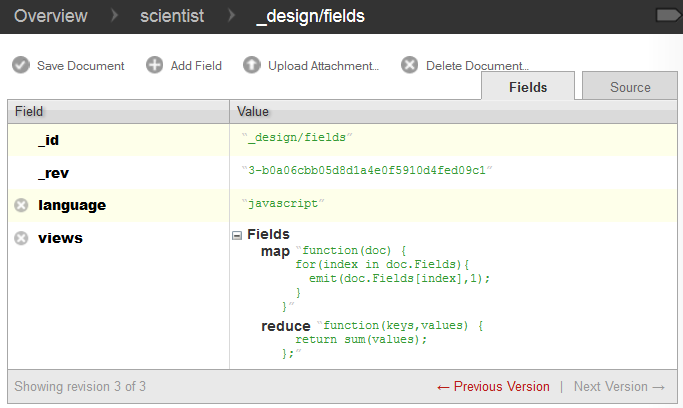
\includegraphics[width=0.65\columnwidth]{images/couchdbviewdocument.png}
\caption{A CouchDB view as a Design document}
\label{img:couchdbviewdocument}
\end{figure}

\begin{figure}[h!]
\centering
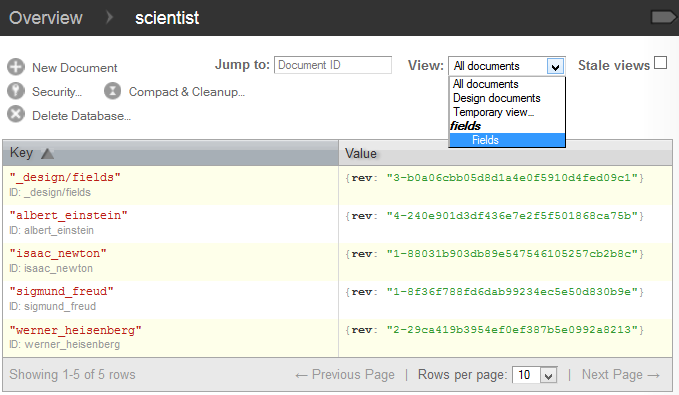
\includegraphics[width=0.65\columnwidth]{images/couchdbviewselection.png}
\caption{Selection of the stored view "Fields" in CouchDB's Futon}
\label{img:couchdbviewselection}
\end{figure}

Design documents are basically common CouchDB documents, however, they may have a special purpose for the CouchDB. This means, although they are stored like common data, they fulfill special roles, e.g. defining queries (as mentioned in the previous Section) or defining CouchApps (see Chapter\~ref{couchapp}). To differentiate common documents from Design documents, the value of each Design document's \emph{\_id} attribute starts with the "\_design\/" prefix.
